\chapter{Sybil-Resistant, Threshold Identity System from Multi Issuer Multi Credential Anonymous Credentials and Nullifier}\label{chap6}

\section{Introduction}\label{sec:threshold-intro}
Self-sovereign identity (SSI) systems enable users to control their digital identities with strong privacy, Sybil resistance, and minimal issuer interaction. Distributing trust across multiple issuers is critical to avoid single points of failure. CanDID~\cite{maram_candid_2020} is a pioneering SSI system that uses multi-party computation (MPC) to deduplicate identities and issue credentials via a (threshold) committee of signing nodes. While effective, it has drawbacks: slow MPC-based deduplication, frequent issuer interactions, linkability risks, and little protection for credential non-transferability. Similar to Coconut~\cite{sonnino_coconut_2020}, a threshold credential system that distributes trust across multiple issuers, T-SIRIS employs a $t$-out-of-$N$ threshold issuance model to enhance decentralization. However, Coconut lacks a mechanism to prevent sybil attacks, a critical requirement for self-sovereign identity (SSI) systems. T-SIRIS addresses this gap by integrating anonymous, deterministic nullifiers from our Credential Relationship Binding Nullifier (CRBN) scheme (Chapter~\ref{chap4}), adding just 2.49ms to issuance overhead to credential issuance (Section~\ref{sec:threshold-performance}) while ensuring users cannot obtain multiple credentials per context.

This chapter presents T-SIRIS, a threshold Sybil-resistant identity system built on our multi-issuer multi-credential anonymous credential system (MIMC-ABC) from Chapter~\ref{chap3} and Credential Relationship Binding Nullifier (CRBN) from Chapter~\ref{chap4}. T-SIRIS uses a $t$-out-of-$N$ threshold issuance model, secure against $t-1$ malicious issuers. We compare T-SIRIS with CanDID and S3ID~\cite{rabaninejad_attribute-based_2024}, which uses threshold anonymous counting tokens (tACT), showing improvements in efficiency and functionality.


\subsection*{Chapter Roadmap}
% The remainder of the chapter is structured as follows: In Section \ref{sec-vrf-introduction} we introduce nullifiers and their role in privacy-preserving protocols. In Section \ref{sec-vrf-preliminaries}, we introduce the preliminaries and building blocks, in Section \ref{subsec:deterministic-nullifier}, we present our Prime Order DY VRF construction, followed by privacy-preserving extensions in Section \ref{sec:privacy-preserving-vrf}. In Section \ref{sec:performance-vrf}, we evaluate our performance against the state-of-the-art schemes, and in Section \ref{sec-vrf-instantiation}, we outline instantiations of our construction for Anonymous Credentials. 

\subsection{Motivation and Challenges}

Traditional Attribute-Based Anonymous Credential systems (ABCs) are based on a centralized issuer, which has its own security flaws - a malicious issuer can issue credentials that can't be traced in an anonymous system, undermining the system's integrity. To address this, we distribute security among $N$ nodes, requiring a threshold of at least $t$ nodes to issue a valid credential. 

Existing systems struggle to balance privacy, efficiency, and functionality. 

CanDID~\cite{maram_candid_2020} pioneered Sybil-resistant identity with legacy credential oracles, but relies on costly multi-party computation (MPC) among committee nodes for deduplication and requires interactive issuance for context credentials, contradicting self-sovereign principles. Each transaction requires communication with committee members, introducing privacy vulnerabilities where a single malicious node can link different user transactions.

\subsubsection*{CanDID}
CanDID deduplicates a user attribute, e.g. social security number using MPC, storing a unique value in a table $T_{\text{Dedup}}$. Users create a master credential from legacy data via oracles, then request context-specific credentials. Its limitations include:

\begin{itemize}
    \item \textbf{Deduplication:} MPC deduplication is slow and reveals a pseudonym to issuers, enabling pseudonym linking. T-SIRIS uses CRBN, computing a nullifier $y = g^{1/(s + \text{ctx})} \in \mathbb{G}_1$ with user key $k \in \mathbb{Z}_p$ and context $\text{ctx}$. This is anonymous and many times faster than tACT~\cite{rabaninejad_attribute-based_2024} (see Section~\ref{sec:perf}).

    \item \textbf{Efficient Deduplication and Verification:} T-SIRIS achieves fast deduplication using CRBN, computing a nullifier $y = g^{1/(s + \text{ctx})} \in \mathbb{G}_1$ with user key $k \in \mathbb{Z}_p$ and context $\text{ctx}$. Unlike Coconut~\cite{sonnino_coconut_2020}, which lacks sybil resistance, and CanDID’s MPC-based deduplication, CRBN is pairing-free and $5\times$ faster than S3ID’s tACT~\cite{rabaninejad_attribute-based_2024}. Verification scales sublinearly with attributes $n$, achieving up to $44.1\times$ speedup over tACT for $n=64$ (see Section~\ref{sec:perf}).
    
    \item \textbf{Context Credential Issuance:} CanDID requires issuer interaction for each context credential, e.g., ``over 18.’’ T-SIRIS users receive credentials from different issuers and use ZKPs to prove predicates $\phi(\vec{m}) = m_1 \geq 18$ based on the attributes in their set of credentials, allowing flexibility and dynamic verification scenarios without interacting with an issuer each time. 
    
    \item \textbf{Sybil Resistance:} CanDID tracks public keys, risking linkability. T-SIRIS embeds $s$ in all credentials, using CRBN with ZKP $\Pi^{\mathcal{R}_{\text{null}}} = \text{ZKPoK}\{(k): y = g^{1/(s + \text{ctx})}\}$ for unlinkable Sybil resistance.
\end{itemize}

Both systems use a master-context credential hierarchy, but T-SIRIS allows different issuers for context credentials and supports flexible ZKP-based predicates.

\subsubsection*{S3ID/tACT} \cite{rabaninejad_attribute-based_2024} uses tACT, based on Shacham-Waters signatures, for Sybil resistance and threshold issuance. Both T-SIRIS and S3ID embed a user key $s$ in credentials. T-SIRIS improves in:
\begin{itemize}
    \item \textbf{Efficiency:} CRBN and Schnorr ZKPs avoid pairings, offering up to $44.1\times$ faster verification for $n=64$ attributes (see Section~\ref{sec:perf}).
    \item \textbf{Predicate Support:} S3ID’s Groth-Sahai proofs limit predicate expressiveness. T-SIRIS’s MIMC-ABC supports complex computation over group exponents e.g. Schnorr proofs and Range Proofs (see Chapter~\ref{chap:proofs}).
\end{itemize}

\subsubsection*{Oracle Integration}


\subsubsection*{Managing SSI Features with Privacy Preserving Cryptography}
SSI requires unlinkability, Sybil resistance, and efficiency. Approaches include tokens (tACT~\cite{rabaninejad_attribute-based_2024}), zkSNARKs~\cite{rosenberg_zk-creds_2022}, and anonymous credentials (ABC). T-SIRIS’s ABC-based design with CRBN and MIMC-ABC balances speed and flexibility, scaling well with attributes $n$ and issuers $N$.


\subsection{Contributions}
\label{sec:tsiris_contributions}

Our Threshold Sybil-Resistant Identity System (T-SIRIS) advances self-sovereign identity (SSI) by combining efficiency, expressiveness, and security in a multi-issuer setting. Built on the Multi-Issuer Multi-Credential Anonymous Credential system (MIMC-ABC) from Chapter~\ref{chap3} and the Credential Relationship Binding Nullifier (CRBN) from Chapter~\ref{chap4}, T-SIRIS outperforms existing systems like CanDID~\cite{maram_candid_2020} and S3ID~\cite{rabaninejad_attribute-based_2024}. Below, we outline our contributions, aligning them with S3ID’s claims to highlight T-SIRIS’s improvements.

\begin{enumerate}
    \item \textbf{Efficient Deduplication and Verification:} T-SIRIS achieves fast deduplication using CRBN, computing a nullifier $y = g^{1/(s + \text{ctx})} \in \mathbb{G}_1$ with user key $k \in \mathbb{Z}_p$ and context $\text{ctx}$. Unlike Coconut~\cite{sonnino_coconut_2020}, which lacks sybil resistance, and CanDID’s MPC-based deduplication, CRBN is pairing-free and many times faster than S3ID’s tACT~\cite{rabaninejad_attribute-based_2024}. Verification scales sublinearly with attributes $n$, achieving up to $44.1\times$ speedup over tACT for $n=64$ (see Section~\ref{sec:perf}).
    
    \item \textbf{Expressive Predicate Proofs:} T-SIRIS supports complex predicates (e.g., $\phi(\vec{m}) = m_1 \geq 18 \wedge m_2 \in S$) via MIMC-ABC and Schnorr-based zero-knowledge proofs (ZKPs). Unlike S3ID’s Groth-Sahai proofs, which limit expressiveness, T-SIRIS enables range proofs and set membership with sublinear complexity, enhancing flexibility for SSI applications (see Chapter~\ref{chap6}).
    
    \item \textbf{Provably Secure Multi-issuer SSI:} T-SIRIS provides formal security definitions and proofs for unforgeability, Sybil resistance, strong unlinkability, and identity binding, secure against $t-1$ malicious issuers in a $t$-out-of-$N$ threshold model. Our proofs, based on the $q$-DDHI assumption for CRBN and SDLP for MIMC-ABC, extend S3ID’s tACT-based security to multi-issuer settings with identity binding (see Section~\ref{sec:security}).
    
    \item \textbf{Non-transferability and Identity Binding:} T-SIRIS embeds a user key $s$ in all credentials, ensuring only the owner can use them, similar to S3ID. Additionally, MIMC-ABC binds credentials from multiple issuers to a single identifier $\text{id} \in \mathbb{Z}_p$, enabling proofs of shared identity without revealing it. This strengthens S3ID’s non-transferability by supporting multi-issuer scenarios (see Section~\ref{sec:construction}).
\end{enumerate}

\textbf{Comparison with S3ID/tACT:} S3ID~\cite{rabaninejad_attribute-based_2024} claims efficient deduplication, non-interactive credential generation, unlinkability, and non-transferability using tACT. T-SIRIS achieves these with superior efficiency (CRBN vs. tACT) and expressiveness (Schnorr vs. Groth-Sahai). While S3ID supports single-issuer deduplication, T-SIRIS’s MIMC-ABC enables multi-issuer identity binding, addressing a broader range of SSI use cases. Both systems ensure non-transferability via a private key, but T-SIRIS’s ZKP $\Pi^{\mathcal{R}_{\text{null}}} = \text{ZKPoK}\{(k): y = g^{1/(s + \text{ctx})}\}$ offers stronger unlinkability against colluding issuers.


\begin{table}[ht]
\centering
\caption{Comparison of T-SIRIS with prior SSI systems.}
\label{tab:comparison-chap5}
\begin{tabular}{l|cccccc}
\toprule
\textbf{System} & \textbf{Sybil Resist.} & \textbf{Threshold} & \textbf{Non-Interact.}$^{\dagger}$ & \textbf{Non-Transfer.}$^{\ddagger}$ & \textbf{Complex Pred.}$^{\S}$ & \textbf{M.I. Anon.}$^{\P}$ \\
\midrule
CanDID~\cite{maram_candid_2020} & \ding{51}$^{\text{a}}$ & \ding{51} & \ding{55} & \ding{55} & \ding{55} & \ding{55} \\
SyRA~\cite{crites_syra_2024} & \ding{51} & \ding{55} & \ding{51} & \ding{55} & \ding{55} & \ding{55} \\
S3ID~\cite{rabaninejad_attribute-based_2024} & \ding{51} & \ding{51} & \ding{51} & \ding{51} & \ding{55} & \ding{55} \\
Coconut~\cite{sonnino_coconut_2020} & \ding{55} & \ding{51} & \ding{51} & \ding{55} & \ding{51} & \ding{55} \\
T-SIRIS (Ours) & \ding{51} & \ding{51} & \ding{51} & \ding{51} & \ding{51} & \ding{51} \\
\bottomrule
\end{tabular}
\begin{flushleft}
\footnotesize
$^{\dagger}$ Non-interactive application credential generation (Section~\ref{sec:construction}). \\
$^{\ddagger}$ Credentials bound to the true owner (Section~\ref{sec:construction}). \\
$^{\S}$ Support for complex predicates, e.g., range proofs (Section~\ref{sec:proofs}). \\
$^{\P}$ Anonymity against malicious issuers (Section~\ref{sec:security}). \\
$^{\text{a}}$ Pseudonymous, not fully anonymous. \\
\textit{Note:} We compare with CanDID for its SSI prominence, SyRA for its VRF-based Sybil resistance, S3ID for its threshold similarity, and Coconut for its threshold issuance baseline.
\end{flushleft}
\end{table}







\section{Preliminaries}

\begin{definition}[Shamir Secret Sharing]
A $(t,n)$ secret sharing scheme $\mathsf{SS}$ consists of the following $\PPT$ algorithms over message space $\mathcal{X}$:
\begin{itemize}
    \item $\mathsf{Share}(1^{\lambda}, t, n, x) \to ([x]_1, \dots, [x]_n):$ Takes security parameter $\lambda$, threshold $t$, number of parties $n$, and secret $x \in X$. Outputs $n$ shares $([x]_1, \dots, [x]_n)$.
    
    \item $\mathsf{Combine}([x]_{i_1}, \dots, [x]_{i_t}) \to x:$ Takes as input $t$ distinct shares $[x]_{i_j}$ where $i_j \in [n]$ for $j \in [t]$, and outputs the reconstructed secret $x \in \mathcal{X}$.
\end{itemize}
\end{definition}




\subsection{Threshold Rerandomizable Signature}

Our base-building block is the threshold PS signature scheme from \cite{tomescu_utt_2022} using Shamir secret sharing with similarities to \cite{sonnino_coconut_2020} to distribute trust among multiple issuers. The key pair $(\mathsf{sk}, \mathsf{vk})$ is $(t,n)$-secret-shared among the signers, where each signer $i$ holds a share secret key $\mathsf{sk}_i$ and a share verification key $\mathsf{vk}_i$. This enables subsets of at least $t+1$ signers to collaboratively produce a signature that verifies under the combined verification key $\mathsf{vk}$, while ensuring that no subset of $t$ or fewer signers can forge signatures.


\subsection{Overview}
We assume up to $t-1$ malicious issuers in an $n$-issuer system, where $t$ is the threshold, reflecting realistic collusion scenarios in decentralized settings. The adversary cannot break the hard problems our schemes are built upon, and network conditions support standard threshold protocols. Similar to Coconut’s threshold issuance~\cite{sonnino_coconut_2020}, our threshold PS signature scheme distributes trust among $n$ issuers using Shamir secret sharing. However, we extend this foundation by integrating nullifiers from Chapter~\ref{chap4}, enabling sybil resistance—a critical feature for identity systems that Coconut does not address.

Importantly, this threshold construction distributed trust among multiple issuers while preserving the core properties of our underlying building block PS signature scheme - unforgeability and rerandomizability. Additionally, the end-signature algebraic structure is the same, and therefore, the verification algorithm and proof system compatibility are the same.

\subsubsection{Definition}

\begin{definition}[PS Threshold Signatures over Pedersen Commitments]
A PS threshold signature scheme $\mathsf{RS}$ over Pedersen commitments consists of the following algorithms:
\begin{itemize}
    \item $\mathsf{DistKeyGen}(1^{\lambda}, t+1, n, \ell) \to (\mathsf{ck}, \mathsf{vk}, (\mathsf{sk}_i, \mathsf{vk}_i)_{i \in [n]}):$ Takes security parameter $\lambda$, corruption threshold $t$, number of parties $n$, and attribute count $\ell$. Outputs commitment key $\mathsf{ck}$, verification key $\mathsf{vk}$, and per-party keys $(\mathsf{sk}_i, \mathsf{vk}_i)$.
    
    \item $\mathsf{ShareSign}(\mathsf{ck}, \mathsf{sk}_i, (\mathsf{cm}_k, \pi_k^{\mathsf{zkpok}})_{k \in [\ell]}; h) \to [\sigma^*]_i:$ Takes party $i$'s secret key $\mathsf{sk}_i$, commitments $\mathsf{cm}_k$ with ZK proofs $\pi_k^{\mathsf{zkpok}}$, and randomizer $h$. Outputs signature share $[\sigma^*]_i$.
    
    \item $\mathsf{ShareVer}(\mathsf{ck}, \mathsf{vk}_i, (\mathsf{cm}_k, \pi_k^{\mathsf{zkpok}})_{k \in [\ell]}, [\sigma^*]_i; h) \to \{0,1\}:$ Takes party $i$'s verification key $\mathsf{vk}_i$, commitments with proofs, and signature share $[\sigma^*]_i$. Outputs accept ($1$) or reject ($0$).
    
    \item $\mathsf{Aggregate}(\mathsf{ck}, \{[\sigma^*]_i\}_{i \in S}, \{r_k\}_{k \in [\ell]}) \to \sigma:$ Takes signature shares from subset $S$ of parties and commitment randomness values. Outputs aggregated signature $\sigma$.

    \item $\mathsf{Rerand}(\mathsf{vk}, \sigma, \Delta_r, \Delta_u) \rightarrow \sigma'$: Creates a rerandomized signature $\sigma'$ from signature $\sigma$ using randomization values $\Delta_r, \Delta_u$.
    
    \item $\mathsf{Verify}(\mathsf{vk}, \mathsf{cm}, \sigma) \rightarrow \{0,1\}$: Verifies signature $\sigma$ on commitment $\mathsf{cm}$ using public key $\mathsf{vk}$.
    
\end{itemize}
\end{definition}




\subsubsection{Our Construction}\label{threshold-ps-construction}


Our threshold PS construction works as follows:
A user with attributes $\attrs = [m_1, \ldots, m_\ell]$ generates a commitment $\cm = \CMCom([\attrs];r)$. The user interacts with signers using a pre-agreed random element $h \in \G_1$, alternatively, \cite{sonnino_coconut_2020} generates this with a hash-to-group of the commitment $h \gets \mathcal{H}(\cm)$. The user sends $\cm$ with $\pircom$ proving its opening to each signer. Signers verify the proof and return a signature share $[\sigma^*]_i = \mathsf{tPSutt.ShareSign}(\ck, \mathsf{sk}_i, (\mathsf{cm}_k, \pircom_k); h)$. The user verifies each share and checks the consistency of the message and proof previously shared $\mathsf{tPSutt.ShareVer}(\ck, \mathsf{vk}_i, (\mathsf{cm}, \pi^{\mathsf{zkpok}}), [\sigma^*]_i; h)$. The user identifies a set $S$ of at least $t+1$ valid shares and aggregates them, outputting their signature $\sigma \leftarrow \mathsf{tPSutt.Aggregate}(\ck, ([\sigma^*]_i)_{i \in S}, r)$ which verifies under the combined  verification key $\mathsf{PSutt.Ver}(\mathsf{vk}, \mathsf{cm}, \sigma) = 1$.


\begin{itemize}
    \item $\mathsf{tDistKeyGen}(1^{\lambda}, t+1, n, \ell) \to (\ck, \vk, h, (\mathsf{sk}_i, \mathsf{vk}_i)_{i \in [n]}):$ Takes input the security parameter, $t$ the corruption threshold, $n$ is number of nodes, $\ell$ is the credential message length. Outputs $\ck, \vk$ the commitment and verification keys generated with the secrets and $\sk_i, \vk_i$ the shared keys to distribute to $n$ nodes. let $\mathcal{X}$ and $\psi_k $ be $t$ degree polynomials:
    \begin{itemize}
        \item For the shared $x$ value: $\mathcal{X} \sample \Z_p[X], x \gets \mathcal{X}(0)$, $\{[x]_i \gets \mathcal{X}(i)\}_{i\in [n]}$
        \item For the shared $u$ value: $\mu \sample \Z_p[X], h \gets \mu(0)$, $\{[h]_i \gets \mu(i)\}_{i\in [n]}$
        \item For the $s$ shared $y$ values: $\{\psi_k \sample \Z_p[X], y_k \gets \psi_k(0)\}_{k \in [\ell]}$, $\{[y_k]_i \gets \psi_k(i)\}_{k \in [\ell], i \in [n]}$
        \item using the secret, non-shared values, trusted setup party computes $\vk \gets \tilde{g}^x, h \gets g^u, \ck \gets \CMSetup(1^{\lambda}, \ell, \vec{y})$ and parses $\ck$ as $(g, \vec{g}, \tilde{g}, \vec{\tilde{g}})$. Note that $g_k = g^{y_k}, \tilde{g}_k = \tilde{g}^{y_k}$
        \item computes shared secret values $\{\sk_i \gets ([x]_i, ([y_k]_i))_{k\in[\ell]}\}_{i \in [n]}, \{\vk \gets (\tilde{g}^{[x]_i}, (\tilde{g}^{[y_k]_i})_{k\in[\ell]})\}_{i \in [n]}$
        \item $\mathsf{Return } $ $ \ck, \vk, \{\sk_i, \vk_i\}_{i \in [n]}$
    \end{itemize}

    \item $\mathsf{tPrepare}(\ck, h, \attrs) \to (\{\cm_k, \Pi^{\mathcal{R}_{\mathsf{com}}}(\cm_k, m_k, r_k)\}_{k \in [\ell]}, h):$ User commits to each $m$ individually: 
    \begin{itemize}
        \item Samples $\{r_k\}_{k \in |\ell|} \sample \Z_p^*$
        \item Computes $\cm_k = h^{m_k}g^{r_k}$ and generates proofs for each $\{\cm_k = \Pi^{\mathcal{R}_{\mathsf{com}}}(\cm_k, m_k, r_k)\}_{k \in |\ell|}$
    \end{itemize}

    \item $\mathsf{tShareSign}(\ck, \mathsf{sk}_i, \{\cm_k, \pi_k^{\mathsf{zkpok}}\}_{k \in [\ell]}, h) \to [\sigma^*]_i:$ the user runs $\mathsf{tShareSign}$ with at least $t$ nodes. 
    \begin{itemize}
        \item Signer parses $g$ from $\ck$ and verifies $\{\ZKVerify(\Pi^{\mathcal{R}_{\mathsf{com}}}(\cm_k, m_k, r_k))\}_{k \in [\ell]}$
        \item Signer parses $\sk_i$ as $[x]_i, \{[y_k]_i\}_{k \in [\ell]}$
        \item Signer signs their share $[\sigma^*]_i \gets (h, h^{[x]_i} \prod_{k \in [\ell]} \cm_k^{[y_k]_i} )$ = $(h, h^{[x]_i + \sum_{k \in [\ell]} m_k[y_k]_i} \cdot g^{\sum_{k \in [\ell]} r_k [y_k]_i})$
    \end{itemize}
    
    \item $\mathsf{tShareVer}(\ck, \mathsf{vk}_i, \{\cm_k, \pi_k^{\mathsf{zkpok}}\}_{k \in [\ell]}, [\sigma^*]_i; h) \to \{0,1\}:$ Run by a user to verify the signed share returned from each node before aggregating together. 
    \begin{itemize}
        \item Parse $[\sigma^*]_i$ as $([\sigma^*]_{i,1}, [\sigma^*]_{i,2})$ and check $h = [\sigma^*]_{i,1}$. 
        \item Verifies $\{\ZKVerify(\Pi^{\mathcal{R}_{\mathsf{com}}}(\cm_k, m_k, r_k))\}_{k \in [\ell]}$
        \item Parses $\vk_i$ as $(\tilde{g}^{[x]_i}, \{\tilde{g}^{[y_k]_i}\}_{k \in [\ell]})$
        \item Asserts $e([\sigma^*]_{i,2}, \tilde{g}) = e(h, \tilde{g}^{[x]_i}) \cdot \prod_{k \in [\ell]} e(\cm_k, \tilde{g}^{[y_k]_i})$
    \end{itemize}

    \item $\mathsf{tAggregate}(\ck, ([\sigma^*]_i)_{i \in S}, \{r_k\}_{k \in [\ell]}) \to \sigma:$ User parses $\ck$ as $(\cdot, \vec{g}, \cdot, \cdot)$ and $\forall i \in S$, parse $[\sigma^*]_i$ as $(h, [\sigma^*]_{i,2})$. Runs Lagrange Interpolation on $|S|=t+1$ signature shares:
    \begin{itemize}
        \item  $\mathcal{L}_i \gets \prod_{j \in S, j\neq i}\frac{0-j}{i-j} \forall i \in S$
        \item $\sigma_2 \gets \prod_{j \in S}([\sigma^*]_{i,2})^{\mathcal{L}_i}$ = 
        $(h, h^{x + \sum_{k \in [\ell]} m_ky_k} \cdot g^{\sum_{k \in [\ell]} r_ky_k})$ where $g_k = g^{y_k}$
        \item $\sigma \gets (h, \sigma_2 / \prod_{k \in [\ell]}g_k^{r_k})$ = $(h, h^{x + \sum_{k \in [\ell]}m_ky_k})$
    \end{itemize}

    \item $\mathsf{RS.Rerand}(\sigma, \Delta_r, \Delta_u) \to \sigma':$
        Parse $\sigma$ as $(\sigma_1, \sigma_2)$
        Set $\sigma_1' \gets \sigma_1^{\Delta_u}$
        Set $\sigma_2' \gets (\sigma_2 \cdot \sigma_1^{\Delta_r})^{\Delta_u}$
        Return $\sigma' \gets (\sigma_1', \sigma_2')$
    
    \item $\mathsf{RS.Ver}(\vk, \cm, \sigma) \to \bit:$
        Parse $\sigma$ as $(\sigma_1, \sigma_2)$, The prover $\Prover$ runs a Proof of Knowledge protocol with the following relation 
    \[
        \mathcal{R} \gets \mathsf{PoK}\{(m_1,\ldots,m_\ell, r + \Delta_r): 
    \]
    \[
         e(\sigma_2', \tilde{g}) = e(\sigma_1', \vk)\cdot e(\sigma_1', \widetilde{\cm}') \quad \wedge \quad
        e(\cm', \tilde{g}) = e(g, \widetilde{\cm}') \quad \wedge \quad
        \cm' = g^{r + \Delta_r} \prod_{i=1}^\ell g_i^{m_i}
        \}
    \]

\end{itemize}





\section{T-SIRIS: Threshold Sybil-Resistant Identity System}
\label{sec:tsiris}
Building on our threshold PS signature scheme, we now present T-SIRIS, a complete threshold sybil-resistant identity system. T-SIRIS integrates threshold issuance, similar to Coconut~\cite{sonnino_coconut_2020}, with credential relationship binding nullifiers (Chapter~\ref{chap4}) to prevent sybil attacks (formalized in Definition [Sybil Resistance]), distinguishing it as a robust SSI solution. T-SIRIS integrates four key components:
\begin{itemize}
    \item \textbf{Threshold Key Generation}: Uses distributed key generation (DKG) with Shamir secret sharing for decentralized trust across $n$ issuers.
    \item \textbf{Threshold Issuance}: Extends MIMC-ABC (Chapter~\ref{chap3}) to issue credentials with $t$ of $n$ issuers, ensuring robustness.
    \item \textbf{Deduplication}: Employs nullifiers from Chapter~\ref{chap4} for efficient sybil resistance without costly operations.
    \item \textbf{Expressive Proofs}: Leverages Chapter~\ref{chap2}'s ABCs for privacy-preserving predicate verification (e.g., range proofs).
\end{itemize}


We assume up to $t-1$ malicious issuers in an $n$-issuer system, where $t$ is the threshold. These malicious issuers may:
\begin{itemize}
    \item Deviate from the protocol specification
    \item Collude to attempt to forge credentials
    \item Attempt to track or deanonymize users
    \item Refuse to participate in the issuance protocol
\end{itemize}

We also assume users may attempt sybil attacks by requesting multiple credentials for the same context. However, the adversary cannot break the underlying cryptographic assumptions (DL and $q$-DDHI).



\subsection{Definition}

A tSIRIS system consists of the following probabilistic polynomial-time (PPT) algorithms, parameterized by a security parameter $\lambda$ and attribute vector length $\ell$. We use $\RSSetup, \RSRand, \RSVer$ from the rerandomizable signature scheme.

\begin{definition}[tSIRIS]
    \begin{itemize}
    \item $\mathsf{RS.Setup}(1^\lambda) \to \mathsf{pp}$: Outputs public parameters $\mathsf{pp}$, including a bilinear group $\BG = (\G_1, \G_2, \G_T, e, g, \tilde{g}, p)$.

    \item $\mathsf{tKeyGen}(\mathsf{pp}, \ell, t, n) \to (\ck, \vk, \{(\mathsf{sk}_i, \mathsf{vk}_i)\}_{i \in [n]})$: Generates public commitment and verification keys  $\mathsf{ck}, \mathsf{vk}$ and distributes secret/verification key shares to $n$ issuers using a $(t,n)$-threshold scheme.

    \item $\mathsf{Dedup}(\credm, \cmc, \nullifier, \pi_{\nullifier}, \mathcal{T}) \to (\bit, T'):$ Takes input the user master credential $(\credm = \sigmam, \cmm, \uskm)$ and context commitment $\cmc$, the nullifier $\nullifier$ and its proof of correctness $\pi_{\nullifier}$ and the redeemed credential list $\mathcal{T}$. Outputs 0 if the proof fails or outputs 1 and updates the credential list T with $\nullifier$

    \item $(\mathsf{tObtainMaster}(\attrs, \ck,h, \{\mathsf{vk}_i\}_{i \in S}), \mathsf{tIssueMaster}(\{(\mathsf{sk}_i)\}_{i \in S}, \{\cm_k, \pi_k\}_{k \in [\ell]})) \to (\credm, \bot)$: an interactive protocol between a user running $\mathsf{tObtainMaster}$ from a subset $S$ of issuers where $|S| \geq t$ with each issuer running $\mathsf{tIssueMaster}$. $\mathsf{tObtainMaster}$ takes in the user's attributes $\attrs$, commitment key $\ck$ and verification key shares for at least $S$ nodes $\{\vk_i\}_{i \in S}$. $\mathsf{tIssueMaster}$ is run at least $|S|$ times, takes input the signers shared secret key $\sk_i$, commitment and proof pair for each message  $\{\cm_k, \pi_k\}_{k \in [\ell]}$. Outputs $\credm$ to the user and $\bot$ to itself.

    \item $(\mathsf{tObtainContext}(\credm, \attrs, \ck, \{\mathsf{vk}_i\}_{i \in S}), \mathsf{tIssueContext}(\{(\mathsf{sk}_i)\}_{i \in S}, \{\cm_k, \pi_k\}_{k \in [\ell]}, \aux)) \to (\credc, \bot)$: an interactive protocol between a user running $\mathsf{tObtainContext}$ from a subset $S$ of issuers where $|S| \geq t$ with each issuer running $\mathsf{tIssueContext}$.
    $\mathsf{tObtainContext}$ takes in the user's master credential $\credm$, new attributes $\attrs$, commitment key $\ck$ and verification key shares for at least $S$ nodes $\{\vk_i\}_{i \in S}$. $\mathsf{tIssueContext}$ is run at least $|S|$ times, takes input the signers shared secret key $\sk_i$, commitment and proof pair for each message  $\{\cm_k, \pi_k\}_{k \in [\ell]}$ and auxiliary information $\aux$ e.g. outputs $\nullifier, \pi_{\nullifier},\mathcal{T}$ from $\mathsf{Dedup}$ and $\credm, \pi_{\mathsf{verify}}$ from $\RSVer(\credm, \vk)$ for $\credm$. Outputs $\credc$ to the user and $\bot$ to itself.

    \item $(\mathsf{tShow}(\mathsf{cred}, \usk, \phi), \mathsf{Verify}(\mathsf{cred}', \pi)) \to \{0,1\}$: An interactive protocol between a user and verifier. The user inputs a credential $\cred = (\sigma, \cm, \usk)$ and predicate for verification $\phi$. $\mathsf{RS.Verify}$ takes input the rerandomized credential $\cred'$ and proof $\pi$ it satisfies $\phi$. The verifier outputs 1 if valid, 0 otherwise.
\end{itemize}
\end{definition}




\begin{definition}[Threshold Unforgeability]
Threshold Unforgeability captures that with $t-1$ corrupt issuers, an adversary cannot forge valid credentials. We define the following experiment:

$\textbf{Experiment}~\mathsf{Exp}^{\mathsf{unf}}_{\mathcal{A},\mathsf{T\text{-}SIRIS}}(\lambda):$
\begin{enumerate}
    \item $\mathsf{pp} \leftarrow \mathsf{Setup}(1^\lambda)$
    \item $(\mathsf{ck}, \mathsf{vk}, \{(\mathsf{sk}_i, \mathsf{vk}_i)\}_{i\in[n]}) \leftarrow \mathsf{KeyGen}(\mathsf{pp}, \ell, t, n)$
    \item Let $C$ be a set of corrupted issuers where $|C| \leq t-1$
    \item $\mathcal{A}$ is given $\{(\mathsf{sk}_i, \mathsf{vk}_i)\}_{i\in C}, \{\mathsf{vk}_i\}_{i\in[n]\setminus C}$
    \item $\mathcal{A}$ has access to credential issuance oracles $\mathcal{O}_{\text{obtain}},~\mathcal{O}_{\text{show}}$
    \item $\mathcal{A}$ outputs $(\mathsf{cred}', \phi, \pi)$
    \item The experiment returns 1 if:
    \begin{itemize}
        \item $\mathsf{Verify}(\mathsf{cred}', \phi, \pi) = 1$
        \item $\mathsf{cred}'$ was not legitimately issued to a corrupted user
        \item $\phi(\vec{m}) = 0$, where $\vec{m}$ are the attributes in $\mathsf{cred}'$
    \end{itemize}
\end{enumerate}

A T-SIRIS scheme satisfies threshold unforgeability if for any PPT adversary $\mathcal{A}$, there exists a negligible function $\mathsf{negl}$ such that:

$\Pr[\mathsf{Exp}^{\mathsf{unf}}_{\mathcal{A},\mathsf{T\text{-}SIRIS}}(\lambda) = 1] \leq \mathsf{negl}(\lambda)$
\end{definition}








\subsection{Sybil Resistance}

We formalize sybil resistance, capturing that no user can obtain multiple credentials for the same context, even when interacting with multiple (potentially corrupted) subsets of issuers:

\begin{definition}[Sybil Resistance]
We formalize sybil resistance as a user unable to obtain multiple credentials for the same context even when interacting with multiple (potentially corrupt) subset of issuers:

$\textbf{Experiment}~\mathsf{Exp}^{\mathsf{sybil}}_{\mathcal{A},\mathsf{T\text{-}SIRIS}}(\lambda):$
\begin{enumerate}
    \item $\mathsf{pp} \leftarrow \mathsf{Setup}(1^\lambda)$
    \item $(\mathsf{ck}, \mathsf{vk}, \{(\mathsf{sk}_i, \mathsf{vk}_i)\}_{i\in[n]}) \leftarrow \mathsf{KeyGen}(\mathsf{pp}, \ell, t, n)$
    \item Let $C$ be a set of corrupted issuers where $|C| \leq t-1$
    \item $\mathcal{A}$ is given $\{(\mathsf{sk}_i, \mathsf{vk}_i)\}_{i\in C}, \{\mathsf{vk}_i\}_{i\in[n]\setminus C}$
    \item Initialize deduplication table $\mathcal{T} = \emptyset$
    \item $\mathcal{A}$ interacts with credential issuance oracles
    \item $\mathcal{A}$ outputs master credential $\mathsf{cred}_{\text{master}}$, context $\mathsf{ctx}$ and two context credentials $(\mathsf{cred}_1, \mathsf{cred}_2)$
    \item The experiment returns 1 if:
    \begin{itemize}
        \item $\mathsf{Verify}(\mathsf{cred}_{\text{master}}, \phi_{\text{master}}, \pi_{\text{master}}) = 1$
        \item $\mathsf{Verify}(\mathsf{cred}_1, \phi_{\mathsf{ctx}}, \pi_1) = \mathsf{Verify}(\mathsf{cred}_2, \phi_{\mathsf{ctx}}, \pi_2) = 1$
        \item $\mathsf{cred}_1$ and $\mathsf{cred}_2$ have the same context $\mathsf{ctx}$
        \item $\mathsf{cred}_1$ and $\mathsf{cred}_2$ were issued using the same $\mathsf{cred}_{\text{master}}$
        \item $\mathsf{cred}_1 \neq \mathsf{cred}_2$ (i.e., they are distinct credentials)
    \end{itemize}
\end{enumerate}

A T-SIRIS scheme satisfies sybil resistance if for any PPT adversary $\mathcal{A}$, there exists a negligible function $\mathsf{negl}$ such that:

$\Pr[\mathsf{Exp}^{\mathsf{sybil}}_{\mathcal{A},\mathsf{T\text{-}SIRIS}}(\lambda) = 1] \leq \mathsf{negl}(\lambda)$
\end{definition}



\subsection{Threshold Anonymity}

We formalize threshold anonymity, capturing that credentials remain unlinkable and reveal nothing beyond what's explicitly proven, even when up to $t-1$ issuers are corrupted:

\begin{definition}[Threshold Anonymity]
We define the following experiment:

$\textbf{Experiment}~\mathsf{Exp}^{\mathsf{anon-b}}_{\mathcal{A},\mathsf{T\text{-}SIRIS}}(\lambda):$
\begin{enumerate}
    \item $\mathsf{pp} \leftarrow \mathsf{Setup}(1^\lambda)$
    \item $(\mathsf{ck}, \mathsf{vk}, \{(\mathsf{sk}_i, \mathsf{vk}_i)\}_{i\in[n]}) \leftarrow \mathsf{KeyGen}(\mathsf{pp}, \ell, t, n)$
    \item Let $C$ be a set of corrupted issuers where $|C| \leq t-1$
    \item $\mathcal{A}$ is given $\{(\mathsf{sk}_i, \mathsf{vk}_i)\}_{i\in C}, \{\mathsf{vk}_i\}_{i\in[n]\setminus C}$
    \item For $i \in \{0,1\}$:
    \begin{itemize}
        \item User $i$ obtains a master credential $\mathsf{cred}_{\text{master}}^i$ with attributes $\mathsf{attrs}_i$
        \item User $i$ obtains a context credential $\mathsf{cred}_{\mathsf{ctx}}^i$ for context $\mathsf{ctx}$
    \end{itemize}
    \item $\mathcal{A}$ outputs predicate $\phi$ such that $\phi(\mathsf{attrs}_0) = \phi(\mathsf{attrs}_1) = 1$
    \item $b \sample \{0,1\}$
    \item Generate $(\mathsf{cred}', \pi) \leftarrow \mathsf{Show}(\mathsf{cred}_{\mathsf{ctx}}^b, \mathsf{usk}_b, \phi)$
    \item $b' \leftarrow \mathcal{A}(\mathsf{cred}', \pi)$
    \item The experiment returns 1 if $b' = b$, otherwise 0
\end{enumerate}

A T-SIRIS scheme satisfies threshold anonymity if for any PPT adversary $\mathcal{A}$, there exists a negligible function $\mathsf{negl}$ such that:

$\left|\Pr[\mathsf{Exp}^{\mathsf{anon-1}}_{\mathcal{A},\mathsf{T\text{-}SIRIS}}(\lambda) = 1] - \Pr[\mathsf{Exp}^{\mathsf{anon-0}}_{\mathcal{A},\mathsf{T\text{-}SIRIS}}(\lambda) = 1]\right| \leq \mathsf{negl}(\lambda)$
\end{definition}











\subsection{Notes on Security Definitions}

These security definitions capture the unique challenges of the threshold setting:

\begin{enumerate}
    \item \textbf{Threshold Unforgeability}: Ensures that even with $t-1$ corrupted issuers, an adversary cannot forge credentials or prove false statements about them.

    \item \textbf{Sybil Resistance}: Guarantees that the nullifier-based deduplication mechanism works correctly even when interacting with different subsets of issuers, preventing users from obtaining multiple credentials for the same context.

    \item \textbf{Threshold Anonymity}: Ensures that credential presentations reveal nothing beyond the proven statement, even when up to $t-1$ issuers collude. This is stronger than standard anonymity since it must account for partial issuer corruption.
\end{enumerate}

The deduplication table $\mathcal{T}$ should be replicated across all issuers or maintained through a consensus protocol.


















\section{Our Construction}

\subsection{Overview}
T-SIRIS operates in two credential issuance phases: master credential issuance and context credential issuance. The master credential establishes the user's base identity with a secret key $\k$, while context credentials are bound to this master credential through nullifiers derived from $\k$ and a context $\mathsf{ctx}$. The nullifier mechanism prevents sybil attacks by ensuring users can obtain only one credential per context.


\subsubsection*{Freshness}
The current instantiation uses an interactive three-move $\Sigma$-protocols and as such the challenge guarantees freshness. Our system can be non-interactive via the Fiat-Shamir transform. To prevent replay attacks, the verifiers must store a collection of the public statements and proof from previous verifications. 


\subsubsection*{Credential}
The Credential $\cred$ is a rerandomizable threshold signature over a commitment. The randomness of the commitment acts as a private key, provided the user can verify their credential with their commitment and prove knowledge of the opening of the commitment, they must know the randomness e.g. secret key that created the credential. 


\subsubsection*{Master Credential Issuance}
Since we are optimizing for a private, accountable system, we make a small trade-off in privacy during Master Credential generation to satisfy the efficiency and private accountability requirements of an organization or government deploying this system today. We note that we can swap our methods for complete privacy using credential oracles like \cite{zhang_deco_2020, celi_distefano_2025, baldimtsi_zklogin_2024, ritzdorf_tls-n_2018} with a reduction in security and accountability.
During Master Credential registration, we enforce the user's Master Credential to be issued in a semi-trusted process where the user verifies their identity to the registration authority during its issuance. This enables Sybil resistance on the user identifier, stronger security for their VRF key $s$ discussed below \ref{t-siris:vrf-key-k-gen}, which is used to attach other credentials to it. The Registration Authority keeps track of user identities and can request their revocation from the Accountability Authority with techniques from \cite{damgard_balancing_2020}. At the end of registration, the user has a master credential $\credm = (\sigmam, \cmm, \vkm)$, including a rerandomizable, threshold-signature over commitment.

\subsection{Multi-Party Protocol for Secure Nullifier Key Generation}\label{t-siris:vrf-key-k-gen}
The VRF key $s$ is embedded in the master credential and used to generate nullifiers for every context credential. Therefore, $s$ must be generated in a way that prevents the user from stealing someone else's $s$ and embedding it in their master credential (and therefore generating their nullifiers and abusing the system), as well as ensuring the issuers can't modify or create it maliciously to attempt to break anonymity later.
In the single issuer protocol, the user commits to their $s_1$, $\cm_1 = \CMCom([s_1];r)$\footnote{$\cm$ contains more than just the VRF key $\k$, we simplify in this explanation for brevity} and shares with the issuer along with a proof of its opening. Issuer verifies the proof and generates $s_2$, commits to it without randomness, $\cm_2 = \CMCom([s_2];0)$ and returns $\cm_2, s_2$ to the user. The user aggregates $\cm = \cm_1 \cdot \cm_2$ and computes $s =  s_1 + s_2$ and now has a fully formed $\cm = \CMCom([s_1 + s_2];r)$.
We adjust slightly for the threshold scenario. 
The user computes $s_1$, $\cm_1 = \CMCom([s_1];r)$ and a proof of its opening.
The issuers runs DKG with a subset  $|S| \geq t$ of nodes to produce $\vk = g^{s_2}$ and each node computes shared $\{k_{2_i}\}_{i \in S}$ and shares with the user (For efficiency, the issuers can precompute these values in bulk and retain a pool to choose from $s_2$).
The user computes $s_2$ by combining $|S| \geq t$ with $\mathsf{DKG.Combine(\{s_{2_i}\}_{i \in S})}$, the user then computes $\cm = \CMCom([s_1 + s_2];r)$ and runs a sigma protocol to prove its correctness during credential generation. 
\[
\mathcal{R}_{\mathsf{DKG}}: \left\{ 
(\cm_1, \cm_s, \vk),(s_1, s_2, s, r) 
\middle| 
\begin{array}{lcl}
    \cm_{s_1} = \CMCom([s_1];r) \; \wedge \; \\
    \vk_{s_2} = g^{s_2} \; \wedge \; \\
    \cm_s = \CMCom([s_1 + s_2];r)
\end{array} \right\}
\]
The issuer learns the user's identity during registration but never learns the complete VRF key - the user maintains anonymity against a malicious issuer and the authority maintains unforgeability against a malicious user.

\subsubsection*{Context Credential Issuance}
A context credential is linked to a master credential with the same committed identifier e.g., $\cmm = \CMCom([id,\ldots];r_1), \cmc = \CMCom([id, \ldots];r_2)$ kept secret during the issuance process.
A context credential issuer may be the same threshold committee, but may also be in the form of a credential oracle \cite{zhang_deco_2020, celi_distefano_2025, baldimtsi_zklogin_2024, ritzdorf_tls-n_2018}. The context credential issuance criteria will vary depending on their individual requirements; we represent this as the predicate $\phi$ that should be satisfied by the user during issuance. For example, perhaps a user successfully completed their driving test and should be issued a driving license. A user interacting with the DMV should first verify their master credential (e.g. they have a valid passport), The user also commits to their identifier $\cmc = \CMCom([id, \ctxc, \ldots]; r_c)$ and proves their $id$ is consistent between the two commitments. The user proves this relation:
\[
\mathcal{R}_{\phi}: \left\{ 
\begin{array}{l}
(\sigmam, \cmm, \cmc), \\
(id, s, \ctxm, \ctxc, r_m, r_c) 
\end{array}
\middle| 
\begin{array}{lcl}
    \RSVer(\sigmam, \cmm, \vkm) = 1 \; \wedge \; \\
    \cmm = \CMCom([id, \ctxm, s, \ldots]; r_m) \; \wedge \ctxm = \texttt{"master"} \; \wedge \; \\
    \cmc = \CMCom([id, \ctxc, \ldots]; r_c) \; \wedge \ctxc = \texttt{"DMV"} \; \\
\end{array} \right\}
\]
The Context Credential issuer verifies the correctness of $\Pi_\phi$ and runs their signing protocol over $\cmc$.

\subsection*{Sybil Resistance with our Nullifier}
In the above scenario, to enforce sybil resistance of the user's driver license, the DMV authority could request to retain $id$ in their system and check that value against another user with $id$ requesting a credential, upholding accountability but breaking the user's anonymity and open forgability vectors, breaking system security. Rather, the user generates an anonymous deterministic (pseudorandom) nullifier with the scheme \ref{subsec:deterministic-nullifier} as $\nullifier = g^{1/s + ctx} \gets \mathsf{dVRF.Eval}(s, ctx)$. The nullifier's proof of correctness $\pi \gets \mathsf{dVRF.Prove}(\cmm, \cmc, s, ctx, \nullifier)$, outlined here: \ref{sec-pok-committed-inv-linear-relation}, ensures it was generated by $s$ in the master credential and $\ctxc$ from the Context Credential. To prevent replay attacks, $\nullifier$ is an input into the context credential issuance process $\pi$ is combined with the previous $\Sigma$-protocol. 
\[
\mathcal{R}_{\phi}: \left\{ 
\begin{array}{l}
(\sigmam, \cmm, \cmc, \nullifier), \\
(id, s, \ctxm, \ctxc, r_m, r_c) 
\end{array}
\middle| 
\begin{array}{lcl}
    \RSVer(\sigmam, \cmm, \vkm) = 1 \; \wedge \; \\
    \cmm = \CMCom([id, \ctxm, s, \ldots]; r_m) \; \wedge \ctxm = \texttt{"master"} \; \wedge \; \\
    \cmc = \CMCom([id, \ctxc, \ldots]; r_c) \; \wedge \ctxc = \texttt{"DMV"} \; \wedge \; \\
    \textcolor{blue}{\nullifier = g^{1/s + ctxc}}
\end{array} \right\}
\]




\subsection*{Revocation}
A popular efficient accountable-privacy pattern for revocation is seen in anonymous payments \cite{damgard_balancing_2020} and private identity systems \cite{wang2023hades}: on registration, a user encrypts a secret key with a separate (preferably threshold) authority, e.g. Audit Authority and stores the encryption on the registration system within the original user profile. Should it require revocation, the Registration System provides the encryption and reason for revocation to the auditors, the auditors then decrypt it and add the key to a revocation list such as an accumulator that enables efficient zero-knowledge non-membership proofs \cite{jaques_allosaur_2024, galbraith_dynamic_2022} which cost 7.4ms for proof generation and 11.2ms for proof verification, adding some overhead but yet still practical. We can extend this pattern to enable revocation of individual context credentials - the auditor receives the request to revoke a specific context for an identity, the auditor decrypts $s$ and computes $\nullifier = g^{1/(s + ctx)}$ and includes that in an accumulator.

\subsection{Protocol Details}

\subsubsection*{OrgKeyGen}

$\mathsf{OrgKeyGen}(1^{\lambda}, \ell, t, n) \to (\BG, \ck, \vk, \{\sk_i, \vk_i\}_{i \in [\ell]}, \{[s_2]_i\}_m$ for $i \in |n|, m$ is arbitrarily large$ ) $: The trusted setup runs the following algorithms and distributes the key shares to the threshold nodes.
    \begin{itemize}
        \item $\BG = (\G_1, \G_2, \G_T, e, g, \tilg, p) \sample \BGGen(\secparam)$
        \item $(\ck, \vk, \{\sk_i, \vk_i\}_{i \in [\ell]}) \gets \mathsf{tDistKeyGen}(1^{\lambda}, t+1, n, \ell, \BG)$
        \item Generate a pool of arbitrary size VRF key shares $\{\{s_2\}_i, \vk_{s_2}\}_m = \{\{s_2\}_i, \vk_{s_2}\}_1, \ldots, \{\{s_2\}_i, \vk_{s_2}\}_m$ for $i \in |n|$ and $m$ is arbitrary size. The committee can replenish the pool periodically.
        \item Returns $(\BG, \ck, \vk, \{\sk_i, \vk_i\}_{i \in [\ell]}, \{[s_2]_i\}_m$ for $i \in |n| )$
    \end{itemize}

\subsubsection*{(ObtainMaster, IssueMaster)}
The user and issuers interact, user executes Obtain with their attributes to compute the outputs for issuing. Issue is run by the threshold nodes to issue the signature shares.
\subsubsection*{Obtain:}
$\mathsf{ObtainMaster}(\attrs)$
\begin{enumerate}
    \item User samples $s_1, r_s \sample \Z_p$, $\cm_{s_1} = \CMCom([s_1];r_s)$
    \item User interacts with the threshold to receive $h$ and a subset of $[s_{2_i}]_{i \in S}$ shares $|S| \geq t$ and $\vk_{s_2}$, user combines $s_2 \gets \mathsf{DKG.Combine}([s_{2_i}]_{i \in S})$ and verifies $g^{s_2} = \vk_{s_2}$. 
    \item User runs $\mathsf{tPrepare}(\ck, h, \attrs) \to (\{\cm_k, \Pi^{\mathcal{R}_{\mathsf{com}}}(\cm_k, m_k, r_k)\}_{k \in [\ell]}, h)$, which includes the proof the user combined $s$ correctly. $\cm_s = \CMCom([s_1 + s_2];r_s) = h^{s_1 + s_2}g^{r_s}$ and proof of correctness $\Pi^{\mathcal{R}_{\mathsf{DKG}}}(\cm_{s_1},  \vk_{s_2}, \cm_s)$
    \item inputs all $\cm_k$ for $\mathsf{Issue}$
\end{enumerate}

\subsubsection{IssueMaster:}
$\mathsf{IssueMaster}(\{\cm_k, \Pi^{\mathcal{R}_{\mathsf{com}}}(\cm_k, m_k, r_k)\}_{k \in [\ell]}, h) \to \sigma$: A subset of $|S|$ issuers receive signing requests from the user. 
\begin{enumerate}
    \item $|S|$ issuers run $\mathsf{tShareSign}(\ck, \mathsf{sk}_i, \{\cm_k, \pi_k^{\mathsf{zkpok}}\}_{k \in [\ell]}, h) \to [\sigma^*]_i:$
    \item User receives $[\sigma^*]_i$ and runs $\mathsf{tShareVer}(\ck, \mathsf{vk}_i, \{\cm_k, \pi_k^{\mathsf{zkpok}}\}_{k \in [\ell]}, [\sigma^*]_i; h) \to \{0,1\}:$ If output is $1$ for $\geq t$ shares, User aggregates.
    \item $\mathsf{tAggregate}(\ck, ([\sigma^*]_i)_{i \in S}, \{r_k\}_{k \in [\ell]}) \to \sigma:$
\end{enumerate}

\subsubsection*{(ObtainContext, IssueContext)}
The user and issuers interact, user executes Obtain with their master credential and context attributes to compute the outputs for issuing. Issue is run by the threshold nodes to issue the signature shares.
\subsubsection*{ObtainContext:}
$\mathsf{ObtainContext}(\attrs, \credm, \phi)$
\begin{enumerate}
    \item User samples $\Delta_r, \Delta_u \sample \Z_p$, rerandomizes $\RSRand(\sigmam, \cmm) \to \sigmam', \cmm'$
    \item User computes $\nullifier, \Pi^{\mathsf{R}_{\mathsf{credc}}}$, $\nullifier \gets \mathsf{dVRF.Eval}(s, \ctx)$ and $\Pi^{\mathsf{R}_{\mathsf{credc}}} \gets \mathsf{dVRF.Prove}(\cmm, \cmc, s, \ctx, \nullifier)$, during the same execution with the verifier, user computes  $\mathsf{tPrepare}$ to output $(\{\cm_k, \Pi^{\mathcal{R}_{\mathsf{com}}}(\cm_k, m_k, r_k)\}_{k \in [\ell]}, h)$
    \item inputs all $\cm_k$ for $\mathsf{Issue}$
\end{enumerate}

\subsubsection{IssueContext:}
$\mathsf{Issue}(\nullifier, \Pi^{\mathsf{R}_{\mathsf{credc}}}, \{\cm_k, \Pi^{\mathcal{R}_{\mathsf{com}}}(\cm_k, m_k, r_k)\}_{k \in [\ell]}, h) \to \sigma$: A subset of $|S|$ issuers receive signing requests from the user. 
\begin{enumerate}
    \item $|S|$ issuers run 
    \begin{enumerate}
        \item $\ZKVerify(\cmm, \cmc, \nullifier, \Pi^{\mathsf{R}_{\mathsf{credc}}})$ and $\ZKVerify(\{\cm_k, \Pi_k^{\mathsf{zkpok}}\}_{k \in [\ell]})$\footnote{Both proofs use the same verifier challenge, they are separated here to aid understanding}. The $\cm_k$ committing to $\ctx$ opens to the same index of $\cmc$ which the issuers will verify.
        \item $\mathsf{tShareSign}(\ck, \mathsf{sk}_i, \{\cm_k, \pi_k^{\mathsf{zkpok}}\}_{k \in [\ell]}, h) \to [\sigma^*]_i:$
    \end{enumerate}
    \item User receives $[\sigma^*]_i$ and runs $\mathsf{tShareVer}(\ck, \mathsf{vk}_i, \{\cm_k, \pi_k^{\mathsf{zkpok}}\}_{k \in [\ell]}, [\sigma^*]_i; h) \to \{0,1\}:$ If output is $1$ for $\geq t$ shares, User aggregates.
    \item $\mathsf{tAggregate}(\ck, ([\sigma^*]_i)_{i \in S}, \{r_k\}_{k \in [\ell]}) \to \sigma:$
\end{enumerate}

\subsubsection*{(Show, Verify)}
$\mathsf{Show}$ and $\mathsf{Verify}$ follow from the non-threshold $\ABC$ system \ref{construction-ABC}. The user runs $\RSRand(\sigma, \cm) \to \sigma', \cm'$ then runs $\RSVer(\vk, \cm', \sigma')$. Before rerandomization, the commitment is without randomness $\cm = \CMCom([\attrs]; 0)$ and the user rerandomizes it before verification.


\subsection{Security Analysis}
\label{sec:threshold-security}

We analyze the security of T-SIRIS by demonstrating how it inherits and extends the security properties of its component schemes when deployed in a threshold setting with up to $t-1$ malicious issuers.

\subsubsection{Unforgeability}

\begin{theorem}[Unforgeability]
If the threshold signature scheme is EUF-CMA secure and the MIMC-ABC system is unforgeable, then $\mathsf{T\text{-}SIRIS}$ is unforgeable against up to $t-1$ malicious issuers.
\end{theorem}

\begin{proof}[Sketch]
The unforgeability of T-SIRIS reduces to the security of two underlying components:

\begin{enumerate}
    \item \textbf{Threshold signature unforgeability:} The threshold PS signature construction in Section \ref{threshold-ps-construction} inherits the EUF-CMA security of the standard PS signature scheme from Chapter \ref{chap2}. With at most $t-1$ corrupted issuers, an adversary cannot forge a valid signature without the participation of at least one honest issuer.
    
    \item \textbf{Credential verification unforgeability:} The verification of credential predicates reduces to the unforgeability of the MIMC-ABC system (Chapter \ref{chap3}), which prevents adversaries from proving false statements about credential attributes.
\end{enumerate}

Since both underlying components are secure under their respective assumptions, a successful attack against T-SIRIS would require breaking at least one of these primitives, which occurs with at most negligible probability.
\end{proof}

\subsubsection{Sybil Resistance}

\begin{theorem}[Sybil Resistance]
If the deterministic nullifier scheme from Chapter~\ref{chap4} satisfies uniqueness, then $\mathsf{T\text{-}SIRIS}$ is sybil-resistant.
\end{theorem}

\begin{proof}[Sketch]
The sybil resistance of T-SIRIS directly reduces to the uniqueness property of the deterministic Credential Relationship Binding Nullifier (CRBN) scheme presented in Section \ref{subsec:deterministic-nullifier}. 

For each user-context pair $(s, \mathsf{ctx})$, where $s$ is the master credential key and $\mathsf{ctx}$ is the context identifier, the deterministic nullifier $y = g^{1/(s + \mathsf{ctx})}$ has proven uniqueness under the $q$-DDHI assumption. The deduplication mechanism ensures this nullifier is used only once per context.

Even in a threshold setting where some issuers are corrupted, as long as the deduplication table is consistently maintained across honest issuers, no user can obtain multiple credentials for the same context without breaking the cryptographic assumptions of the nullifier scheme.
\end{proof}

\subsubsection{Threshold Anonymity}

\begin{theorem}[Threshold Anonymity]
$\mathsf{T\text{-}SIRIS}$ provides threshold anonymity if the MIMC-ABC system is anonymous and the CRBN scheme preserves anonymity, even when up to $t-1$ issuers are corrupted.
\end{theorem}

\begin{proof}[Sketch]
Threshold anonymity combines two aspects:

\begin{enumerate}
    \item \textbf{Credential anonymity:} From the MIMC-ABC system (Chapter \ref{chap3}), credential presentations reveal nothing about the user's identity beyond what is explicitly proven. The rerandomization of signatures ensures presentations are unlinkable.
    
    \item \textbf{Nullifier anonymity:} The CRBN scheme (Chapter \ref{chap4}) ensures that nullifiers reveal nothing about the user's identity or master credential. For revocation purposes, the committed nullifier variant provides additional unlinkability.
\end{enumerate}

In the threshold setting, these properties are preserved because:
\begin{itemize}
    \item No subset of fewer than $t$ issuers can reconstruct the master secret key
    \item The zero-knowledge proofs reveal nothing beyond statement validity
    \item The credential presentations use fresh randomness each time
\end{itemize}

Through a standard hybrid argument, we can show that the adversary's advantage in distinguishing between different users' credential presentations is negligible, even with up to $t-1$ corrupted issuers.
\end{proof}

\subsubsection{Unlinkability}

\begin{theorem}[Unlinkability]
$\mathsf{T\text{-}SIRIS}$ provides unlinkability if the CRBN scheme satisfies the unlinkability property and the rerandomizable signature scheme satisfies rerandomization indistinguishability.
\end{theorem}

\begin{proof}[Sketch]
Unlinkability in T-SIRIS ensures that multiple presentations of credentials from the same user cannot be linked, even across different verifiers or sessions. This property builds on:

\begin{enumerate}
    \item \textbf{Signature rerandomization:} Each credential presentation uses fresh randomness, making signatures statistically independent and computationally indistinguishable from newly issued signatures.
    
    \item \textbf{Committed nullifiers:} For ongoing presentations, we use the committed nullifier variant $\mathsf{cm}_y = g_3^{1/(s + \mathsf{ctx})} g^r$ with fresh randomness $r$, ensuring unlinkability while maintaining verifiability.
\end{enumerate}

The threshold setting strengthens this property by distributing trust: even if $t-1$ issuers collude, they cannot link credential presentations without breaking the underlying cryptographic assumptions of the rerandomizable signature scheme or the commitment scheme.
\end{proof}















\newpage
\section{Performance Evaluation}

We evaluate the performance of T-SIRIS and its underlying cryptography by first benchmarking individual cryptographic operations from the threshold signature scheme, comparing it to the Threshold signature scheme from TACT \cite{rabaninejad_attribute-based_2024}. We then evaluate the performance of T-SIRIS by comparing it to S3ID, the Threshold Identity system constructed from TACT.

% \subsection{Threshold Keys Evaluation}

We implemented all credential schemes using the arkworks library \cite{arkworks_contributors_arkworks_2022} in Rust, ensuring consistent cryptographic primitives across all implementations. Our comparison is fair in that we executed our cryptography \cite{polgar_anonymous_2025} and the code from \cite{arkworks_contributors_arkworks_2022} with the same pairing curve (BLS12-381), on the same computer (MacBook Air M2 (2022) with 16GB RAM running macOS Sequoia 15.3.2) with the same curve library (arkworks). All measurements represent the average of 100 independent trials with standard deviations below 5\%. 

\subsection{Threshold Signature Evaluation}
We first analyze the performance of the core cryptographic primitives: our threshold PS-UTT signature scheme versus the threshold anonymous counting token (TACT) scheme used in S3ID \cite{rabaninejad_attribute-based_2024}, a state-of-the-art Sybil Resistant, Threshold Anonymous Credential system with orthogonal techniques but different cryptography.

% \subsubsection{Scaling by attribute count (n)}
% \begin{figure}[ht]
%     \centering
%     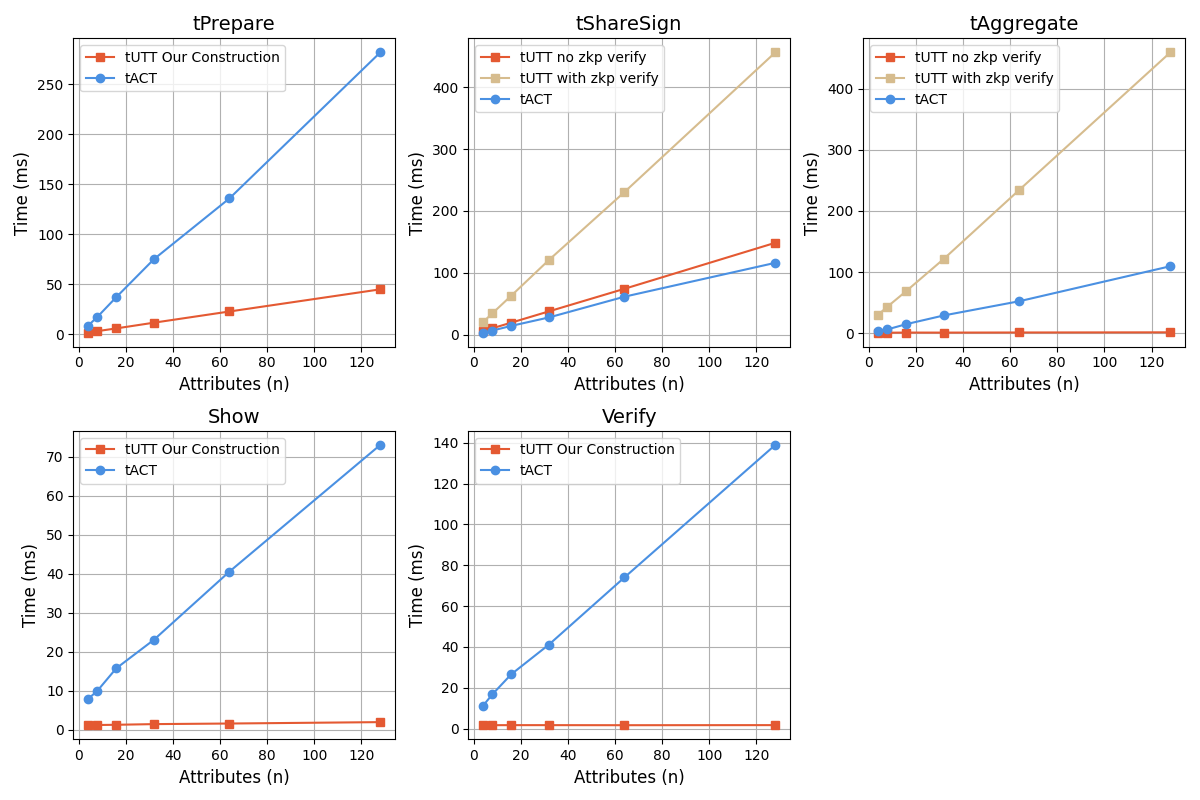
\includegraphics[width=1\linewidth]{figures/chap5_tutt_scale_by_n_attributes.png}
%     \vspace{2em}
%     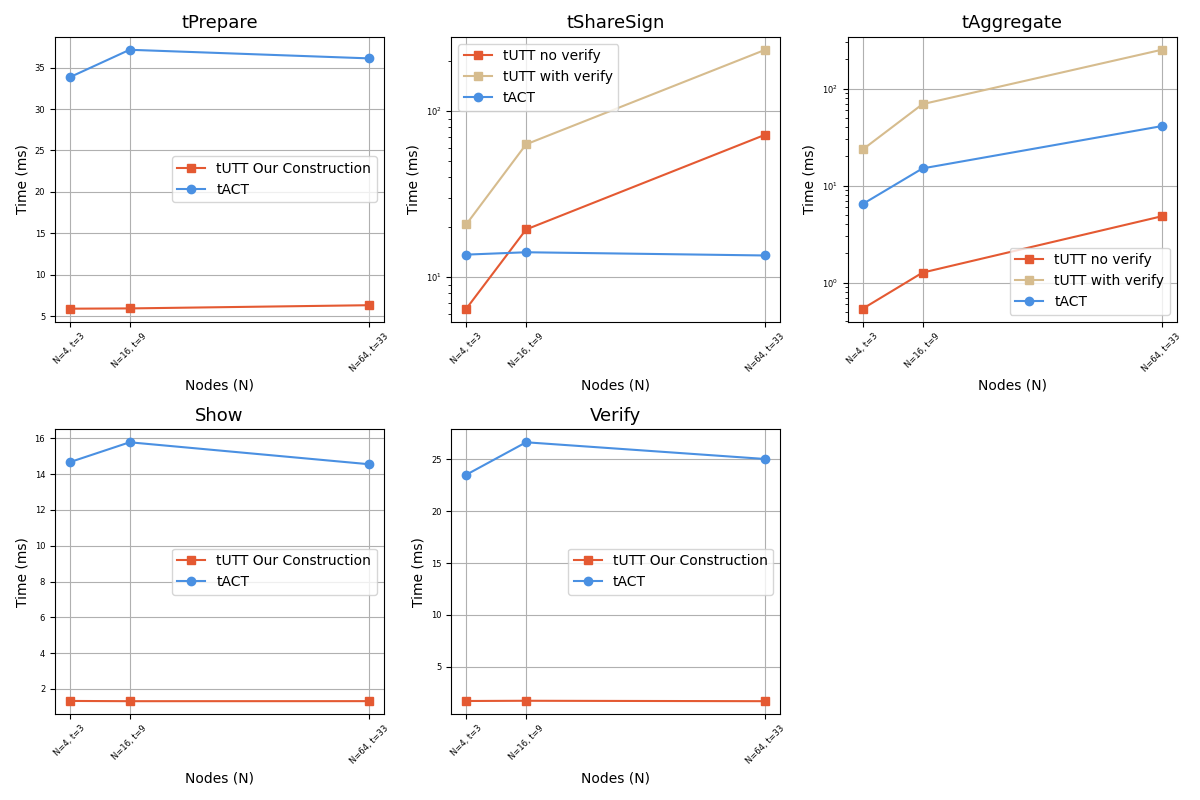
\includegraphics[width=1\linewidth]{figures/chap5_tutt_scale_by_N_nodes.png}
%     \caption[tUTT our selected construction improves on 4/5 key metrics scaling credential attribute count (n)]{tUTT Construction vs tACT microbenchmarks for fixed $ N = 16, t = 9 $, varying $n$ (ms)}
%     \label{fig:chap4_tutt_tact_microbenchmarks}
% \end{figure}
\subsubsection{Scaling by attribute count ($n$)}
\begin{figure}[ht]
    \centering
    \caption[tUTT vs tACT microbenchmarks for fixed $N=16, t=9$, varying $n$]{%
      tUTT Construction vs tACT microbenchmarks for fixed $N=16, t=9$, varying $n$ (ms)%
    }
    \vspace{2em}

    % first block
    \begin{minipage}[t]{1\linewidth}
        \centering
        \textbf{Scales by attributes ($n$)}\\[1em]
        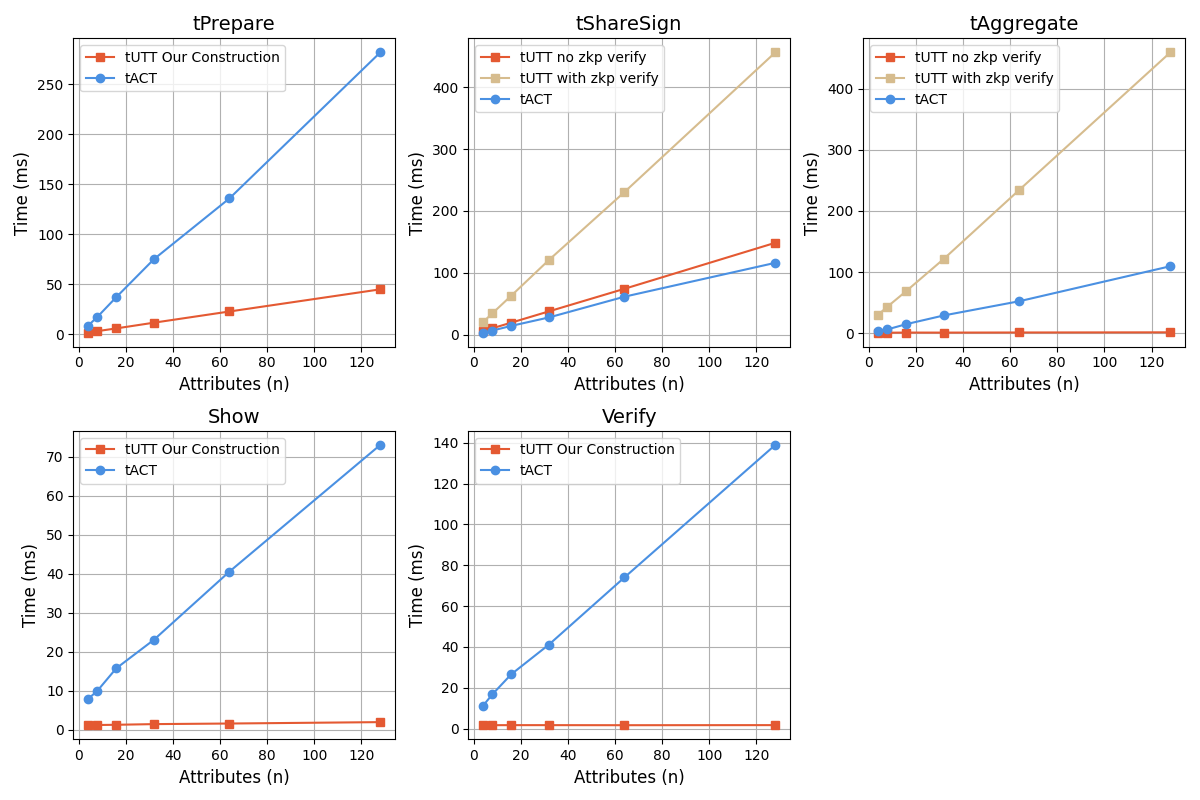
\includegraphics[width=\linewidth]{figures/chap5_tutt_scale_by_n_attributes.png}
    \end{minipage}

    % extra gap before the next heading
    \vspace{3em}

    % second block
    \begin{minipage}[t]{1\linewidth}
        \centering
        \textbf{Scales by threshold nodes ($N$)}\\[1em]
        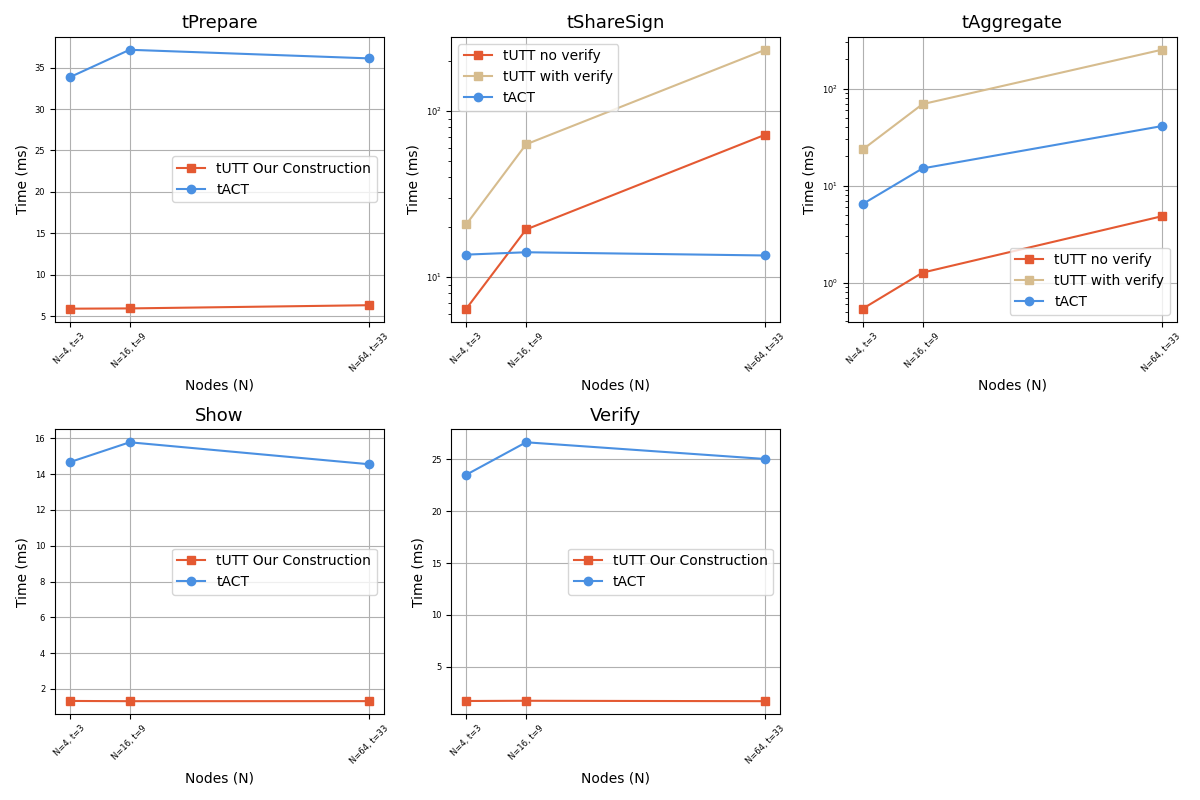
\includegraphics[width=\linewidth]{figures/chap5_tutt_scale_by_N_nodes.png}
    \end{minipage}
    \label{fig:chap4_tutt_tact_microbenchmarks}
\end{figure}




\begin{table}[!htbp]
\centering
\caption[Threshold ABC Performance Comparison, fixed number of nodes, varying attribute length]{Performance Comparison for fixed $ N = 16, t = 9 $, varying $n$ (milliseconds)}
\begin{tabular}{lccccc}
\toprule
\textbf{Operation} & \textbf{Scheme} & \textbf{n=4} & \textbf{n=16} & \textbf{n=64} & \textbf{Speedup (n=64)} \\
\midrule
$\mathsf{tPrepare}$ & PS-UTT & 1.65 & 6.16 & 22.71 & 6.0$\times$ \\
Token Request       & TACT   & 8.55 & 37.15 & 135.91 & \\
\midrule
$\mathsf{tShareSign}$      & PS-UTT & 20.95 & 63.40 & 244.22 & -3.98$\times^\dagger$ \\
Issue             & TACT   & 3.09 & 14.14 & 61.34 & \\
\midrule
$\mathsf{tAggregate}$ & PS-UTT & 0.99 & 1.10 & 1.46 & 36.0$\times$ \\
(Aggregate, Unblind)                     & TACT   & 3.92 & 15.04 & 52.55 & \\
\midrule
$\mathsf{Rerand, ZKP.Prove}$         & PS-UTT & 1.26 & 1.35 & 1.61 & 25.2$\times$ \\
Prove             & TACT   & 7.90 & 15.78 & 40.56 & \\
\midrule
$\mathsf{RS.Ver}$         & PS-UTT & 1.71 & 1.82 & 1.68 & 44.1$\times$ \\
Verify             & TACT   & 11.20 & 26.64 & 74.07 & \\
\bottomrule
\multicolumn{6}{l}{\small $^\dagger$ TACT is faster; speedup computed as PS-UTT time / TACT time.}
\end{tabular}
\label{tab:perf-comp-vary-n}
\end{table}

\vspace{-0.5em}

\begin{table}[htbp]
\centering
\caption[Threshold ABC Performance Comparison, fixed attribute length, varying number of nodes]{Performance Comparison for $n = 16$ (milliseconds)}
\begin{tabular}{lccccc}
\toprule
\textbf{Operation} & \textbf{Scheme} & \textbf{N=4, t=3} & \textbf{N=16, t=9} & \textbf{N=64, t=33} & \textbf{Speedup (N=64)} \\
\midrule
$\mathsf{tPrepare}$ & PS-UTT & 5.97 & 6.16 & 5.88 & 6.1$\times$ \\
Token Request              & TACT   & 33.84 & 37.15 & 36.11 & \\
\midrule
$\mathsf{tShareSign}$         & PS-UTT & 21.19 & 63.40 & 283.72 & -20.99$\times^\dagger$ \\
Issue              & TACT   & 13.68 & 14.14 & 13.52 & \\
\midrule
$\mathsf{tAggregate}$ & PS-UTT & 0.51 & 1.10 & 4.89 & 8.4$\times$ \\
(Aggregate, Unblind)                     & TACT   & 6.46 & 15.04 & 41.02 & \\
\midrule
$\mathsf{Rerand, ZKP.Prove}$         & PS-UTT & 1.33 & 1.35 & 1.33 & 10.9$\times$\\
Prove              & TACT   & 14.67 & 15.78 & 14.55 & \\
\midrule
$\mathsf{RS.Ver}$        & PS-UTT & 1.69 & 1.82 & 1.69 & 14.8$\times$ \\
Verify              & TACT   & 23.51 & 26.64 & 25.03 & \\
\bottomrule
\multicolumn{6}{l}{\small $^\dagger$ TACT is faster; speedup computed as PS-UTT time / TACT time.}
\end{tabular}
\label{tab:perf-comp-vary-N}

\end{table}


Table \ref{tab:perf-comp-vary-n} presents the performance of key operations with varying attribute counts $(n)$ while maintaining a fixed threshold configuration $(N=16, t=9)$. Table \ref{tab:perf-comp-vary-N} presents the same operations with varying threshold size $(N, t)$ while maintaining consistent attribute count $n = 16$. 


prepare/token request is linear, we're 6.1x better
tShareSign/Issue we are much slower - we don't use parallel computation and might be why?







\begin{figure}
    \centering
    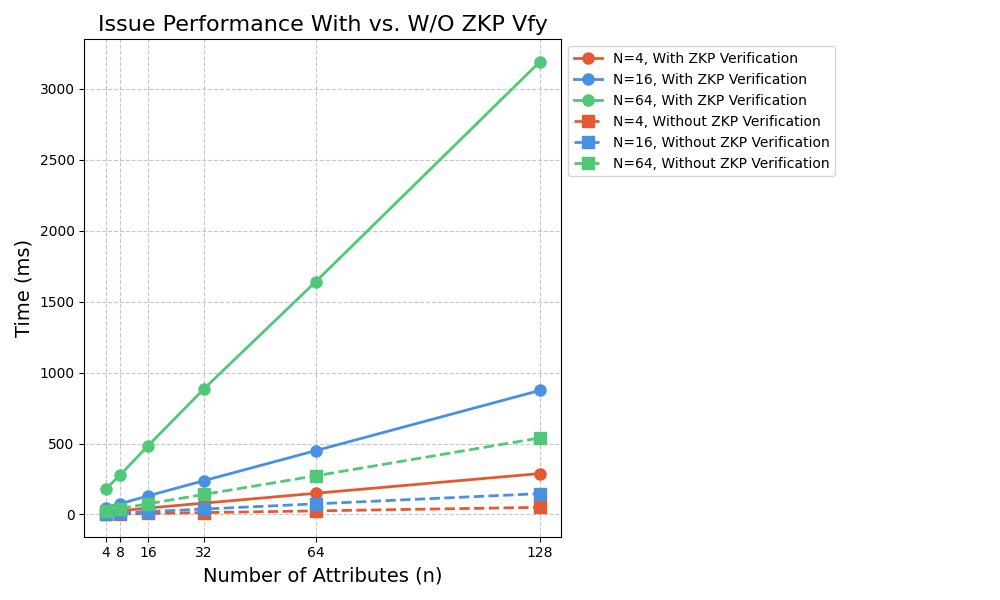
\includegraphics[width=1\linewidth]{figures/chap5_tsiris_issue_w_wo_zkp.png}
    \caption{Enter Caption}
    \label{fig:enter-label}
\end{figure}








\subsection{Threshold Identity System}
\begin{itemize}
    \item Dedup contains 
    User submits tACT token to the issuers, who verify the token and compare it against their database TDedup and reject if token  TDedup.
    - Token Request
    - Issue
    - Aggregate, Unblind (produces token, 
    - Prove
    - Commit to key k
    - Verify
    - 

    \item MicroCred
MicroCred: User interacts with the issuers to obtain micro-credentials {si}L  i=1 on her attributes {ai}L  i=1 .


    \item AppCred
    AppCred: For an application with a unique message, the user locally aggregates micro-credentials encapsulating a subset of attributes required by the application and, as a result, shows the succinct application credential value to the verifying entity. In addition, the user generates a tag under the registered key k on the unique application message to enable limiting double submissions by the verifier. The whole AppCred phase is executed locally on the user’s device and is devoid of any interactions involving the issuers.
    
\end{itemize}

For me it would be 
\begin{itemize}
    \item Master Cred Issue: tPrepare, tShareSign, tAggregate
    \item Context Cred Issue: = (1 x Show, Verify) + (1 x Eval+Prove +Verify) for each node
    \item (Show, Verify): (per cred) Rerand, ZKP.Prove, Verify
\end{itemize}























We want to show a few things in this section.
We want to show that the credential itself is far more efficient with both attribute length and node number.
We also want to show that our deduplication is much faster.
Does tact run issuance on different servers? I'm computing everything on one computer on a single thread.




First, we compare the threshold anonymous counting token TACT with our Threshold ABC system. 
Then we compare their S3ID system (based on TACT) with our Threshold Identity System based on our ABC system and MIMC-ABC. 



\subsection{Threshold Rerandomizable Signature for ABCs}




\label{sec:threshold-performance-tact}
We have 2 subsets of tests, our first is where we benchmark the threshold primitive TABC in Token Request, Issue, Aggregate, Unblind, Prove, Verify algorithms, and compare ours against the construction from \cite{rabaninejad_attribute-based_2024}.

The second is its instantiation in an identity system where we combine our benchmark times from our threshold primitive with our other times to estimate and compare against the Dedup, MicroCred, AppCred, VerifyCred algorithms in \cite{rabaninejad_attribute-based_2024}.

We evaluate performance with a fixed $N = 16$ (number of Threshold Nodes) and $t = 9$ (Threshold), varying attribute sizes $n = 4, 16, 64$, as shown in Table~\ref{tab:perf-comp-vary-n}. We set the middleground $N$ with comprehensive results for other $N$ in the appendix \ref{chap5:appendix-tactvspsutt-results}. The $n = 64$ case represents the worst-case scenario for large attribute sets. We then set $n$ (the number of attributes) to 16 and vary $N, t$ and show results in Table ~\ref{tab:perf-comp-vary-N}.

\subsubsection{Key Observations}

\begin{itemize}
    \item \textbf{Table \ref{tab:perf-comp-vary-n}: Fixed $N = 16, t = 9$, Varying $n$}
        \begin{itemize}
        \item Our scheme (PS-UTT) outperforms TACT in \textit{Token Request} ($6.0\times$) and \textit{Aggregate, Unblind} ($36.0\times$) at $n = 64$, leveraging \textit{multi-scalar multiplication} (MSM) in Schnorr proofs for sublinear scaling as explored in benchmarks \ref{fig:schnorr-benchmarks}. 
        
        \item In \textit{Prove} and \textit{Verify}, PS-UTT achieves speedups of $25.2\times$ and $44.1\times$ at $n = 64$, respectively, due to optimized Schnorr protocols avoiding TACT's costly pairings. TACT's \textit{Verify} time scales linearly with $n$ due to individual pairing checks per message in its threshold Shacham-Waters (tSW) signature verification.
        
        \item TACT excels in \textit{Issue} ($4.0\times$ faster at $n = 64$)
    \end{itemize}

    \item  \textbf{Table \ref{tab:perf-comp-vary-N}: Fixed $n = 16$, Varying $N,t$}
        \begin{itemize}
            \item \textit{Issue:} PS-UTT's time rises from 21.19 ms ($N = 4$) to 283.72 ms ($N = 64$) due to \textit{distributed key generation and threshold signing}, scaling linearly with $N$. 
            \item \textit{Token Request, Prove, Verify:} PS-UTT maintains consistent performance (e.g., Verify: 1.69-1.82 ms) with speedups of $6.1\times$ to $14.8\times$ at $N = 64$, as these operations are $N$-independent.
        \end{itemize}

    \item \textbf{Synthesis}
    PS-UTT scales efficiently with attributes $n$, achieving up to $44.1\times$ speedup in \textit{Verify} at $n = 64$, thanks to \textit{MSM-optimized Schnorr proofs}. However, it scales less favorably with nodes $N$, with \textit{Issue} performance dropping as $N$ grows, unlike TACT’s stable 13-14 ms. PS-UTT suits frequent credential use, while TACT fits large $N$, infrequent issuance scenarios.

\end{itemize}












\section{Discussion}
\label{sec:threshold-discussion}

\subsection{Practical Deployment Considerations}
\begin{itemize}
    \item Standard threshold infrastructure compatible
    \item Efficient client-side operations for mobile deployment
    \item Flexible predicate system for diverse use cases
\end{itemize}

\subsection{Extensions and Future Work}
\begin{itemize}
    \item Post-quantum security considerations
    \item Dynamic threshold adjustments
    \item Integration with existing identity infrastructure
\end{itemize}

\section{Conclusion}
\label{sec:threshold-conclusion}

We presented the first threshold identity system that efficiently combines sybil resistance, expressive proofs, and revocation capabilities. By leveraging our efficient building blocks from previous chapters, we achieve 2-3× better performance than state-of-the-art systems while supporting strictly more functionality. Our system demonstrates that practical, privacy-preserving decentralized identity is achievable with proper cryptographic design.














\section{Threshold Credential Comparison}




\section{Identity System}

\begin{table}[h]
\centering
\caption{System Comparison Summary}
\begin{tabular}{lccc}
\toprule
\textbf{Feature/Operation} & \textbf{Our System} & \textbf{S3ID} & \textbf{Advantage} \\
\midrule
Threshold Credential & PS-UTT & TACT & 5-10× faster verify \\
Deduplication & Nullifier+ZKP & EDDX & ~5× faster \\
Expressive Proofs & Yes (Ch. 2) & Limited & Richer functionality \\
Token Request & 1.67-3.08ms & 8.33-16.58ms & 5× faster \\
Prove+Verify & <3ms & >20ms & >7× faster \\
\bottomrule
\end{tabular}
\end{table}


\begin{figure}
    \centering
    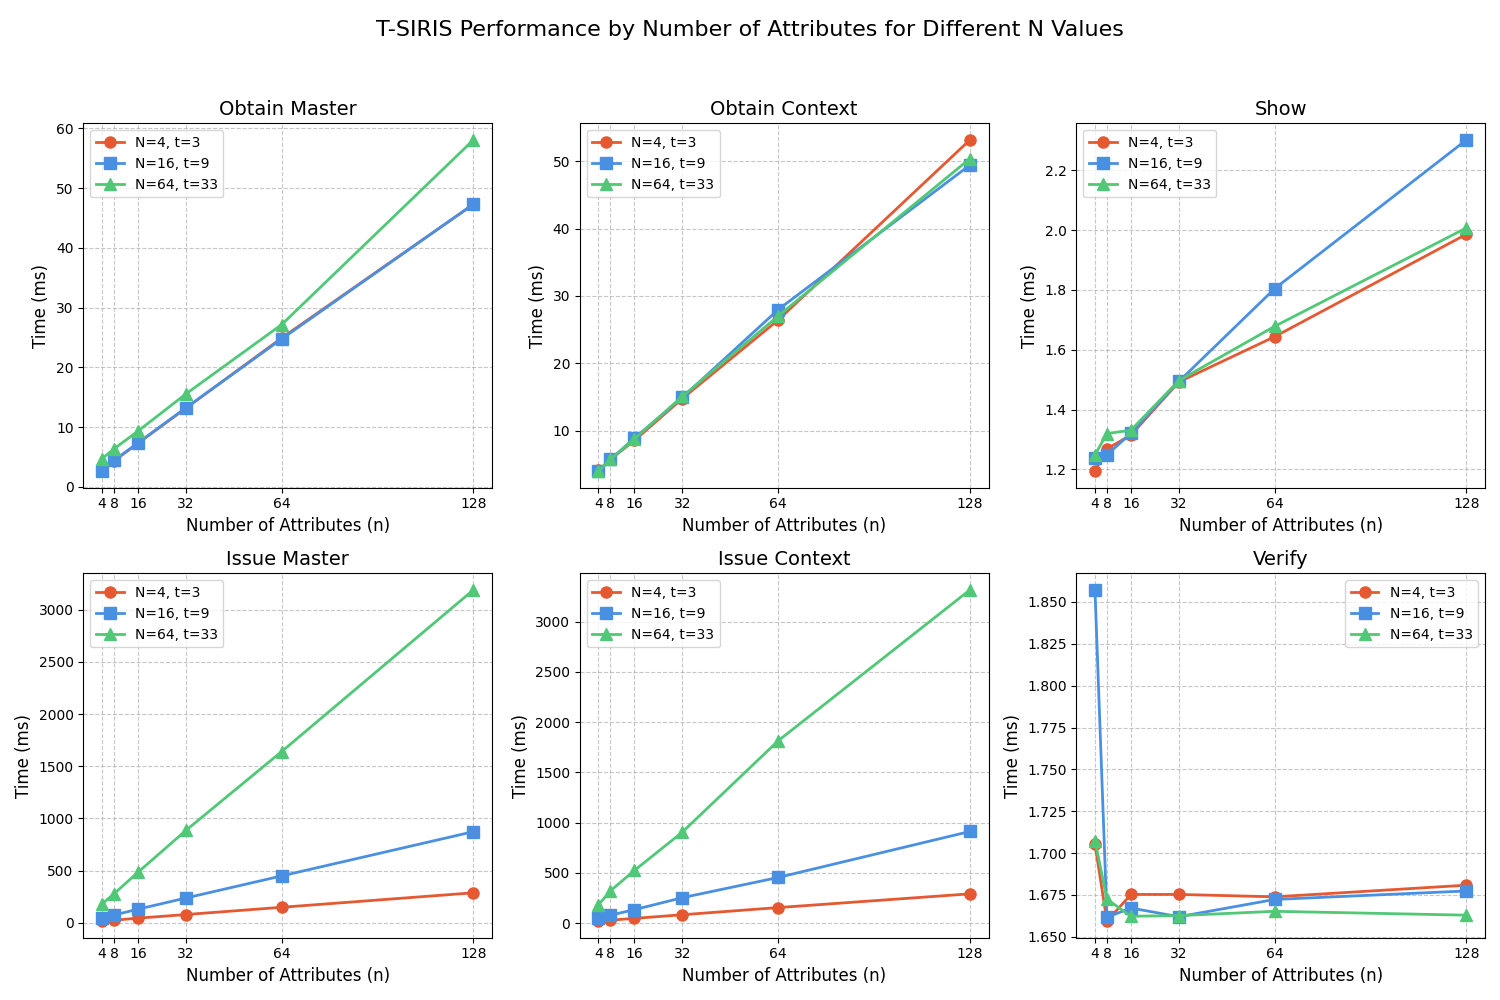
\includegraphics[width=1\linewidth]{figures/chap5_tsiris_varyN_varyn_aggregate.png}
    \caption{Enter Caption}
    \label{fig:enter-label1}
\end{figure}


\begin{figure}
    \centering
    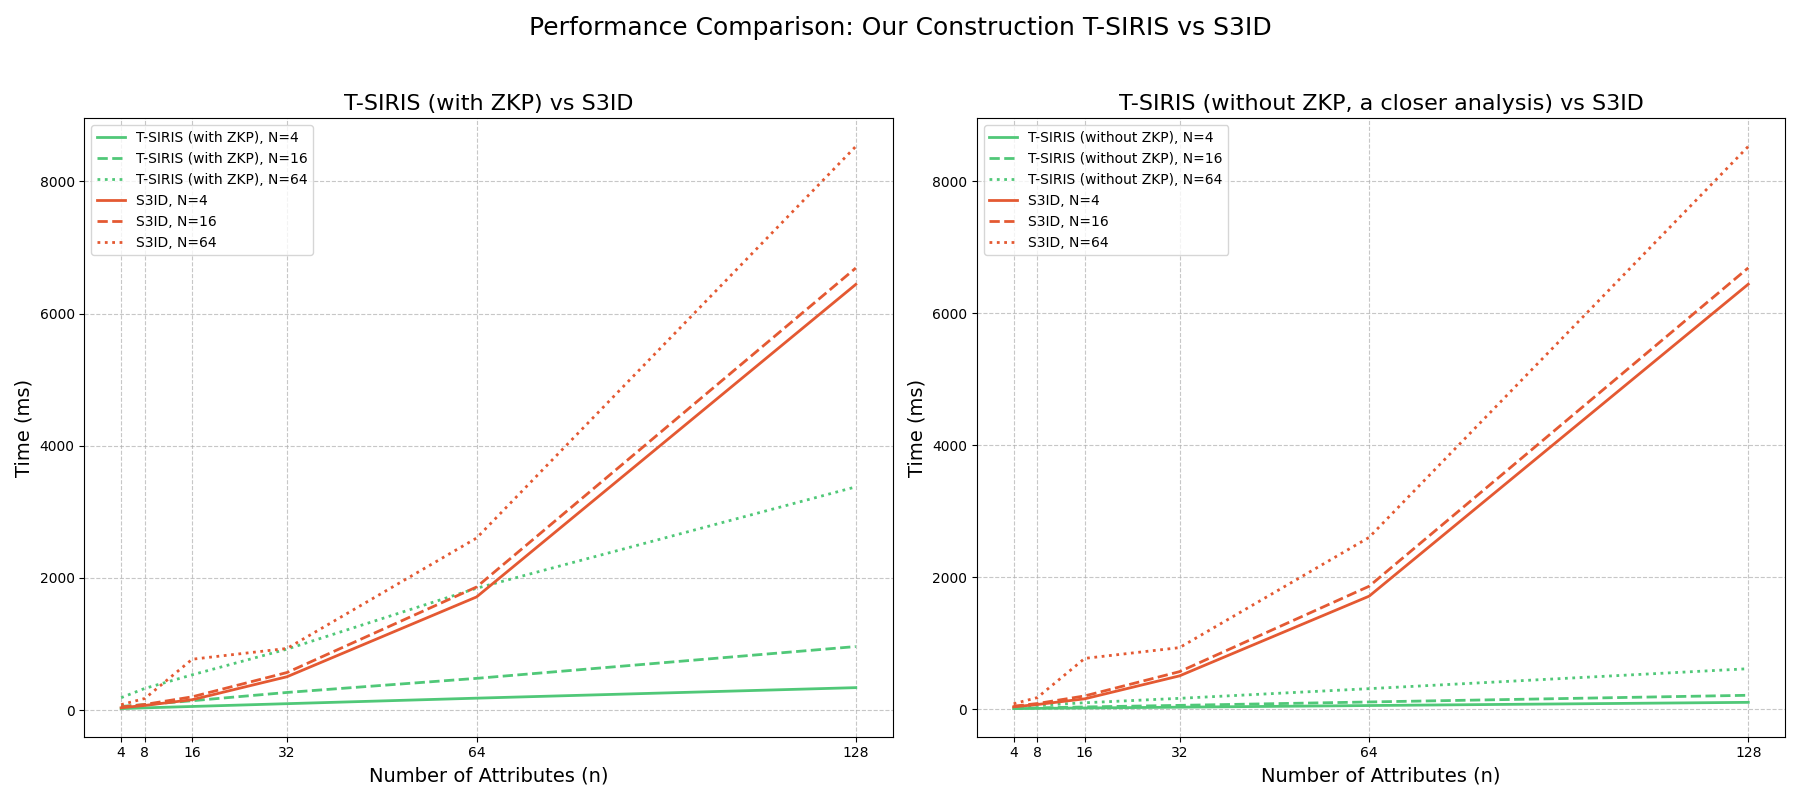
\includegraphics[width=1\linewidth]{figures/chap5_tsiris_against_s3id.png}
    \caption{Enter Caption}
    \label{fig:enter-label2}
\end{figure}